\documentclass{article}

% preamble
\def\npart{III}
\def\nyear{2019}
\def\nterm{Lent}
\def\draft{Ongoing course, rough}
\def\nlecturer{Dr M. Tointon}
\def\ncourse{Introduction to Approximate Groups}

\usepackage{imakeidx}
\usepackage{marginnote}
\usepackage{graphicx}
\usepackage{xfrac}

\ifx \nauthor\undefined
  \def\nauthor{Bhavik Mehta}
\else
\fi

\author{Based on lectures by \nlecturer \\\small Notes taken by \nauthor}
\date{\nterm\ \nyear}
\title{Part \npart\ -- \ncourse}

\usepackage[utf8]{inputenc}
\usepackage{amsmath}
\usepackage{amsthm}
\usepackage{amssymb}
\usepackage{enumerate}
\usepackage{mathtools}
\usepackage{graphicx}
\usepackage[dvipsnames]{xcolor}
\usepackage{tikz}
\usepackage{wrapfig}
\usepackage{centernot}
\usepackage{float}
\usepackage{braket}
\usepackage[hypcap=true]{caption}
\usepackage{enumitem}
\usepackage[colorlinks=true, linkcolor=mblue]{hyperref}
\usepackage[nameinlink,noabbrev]{cleveref}
\usepackage{nameref}
\usepackage[margin=1.5in]{geometry}

% Theorems
\theoremstyle{definition}
\newtheorem*{aim}{Aim}
\newtheorem*{axiom}{Axiom}
\newtheorem*{claim}{Claim}
\newtheorem*{cor}{Corollary}
\newtheorem*{conjecture}{Conjecture}
\newtheorem*{defi}{Definition}
\newtheorem*{eg}{Example}
\newtheorem*{ex}{Exercise}
\newtheorem*{fact}{Fact}
\newtheorem*{law}{Law}
\newtheorem*{lemma}{Lemma}
\newtheorem*{notation}{Notation}
\newtheorem*{prop}{Proposition}
\newtheorem*{question}{Question}
\newtheorem*{rrule}{Rule}
\newtheorem*{thm}{Theorem}
\newtheorem*{assumption}{Assumption}

\newtheorem*{remark}{Remark}
\newtheorem*{warning}{Warning}
\newtheorem*{exercise}{Exercise}

% \newcommand{\nthmautorefname}{Theorem}

\newtheorem{nthm}{Theorem}[section]
\newtheorem{nlemma}[nthm]{Lemma}
\newtheorem{nprop}[nthm]{Proposition}
\newtheorem{ncor}[nthm]{Corollary}
\newtheorem{ndef}[nthm]{Definition}

% Special sets
\newcommand{\C}{\mathbb{C}}
\newcommand{\N}{\mathbb{N}}
\newcommand{\Q}{\mathbb{Q}}
\newcommand{\R}{\mathbb{R}}
\newcommand{\Z}{\mathbb{Z}}

\newcommand{\abs}[1]{\left\lvert #1\right\rvert}
\newcommand{\norm}[1]{\left\lVert #1\right\rVert}
\renewcommand{\vec}[1]{\boldsymbol{\mathbf{#1}}}

\let\Im\relax
\let\Re\relax

\DeclareMathOperator{\Im}{Im}
\DeclareMathOperator{\Re}{Re}
\DeclareMathOperator{\id}{id}

\definecolor{mblue}{rgb}{0., 0.05, 0.6}

\usepackage{tikz-cd}
\newcommand{\vge}{\rotatebox[origin=c]{-90}{$>$}}
\newtheorem{nthm*}[nthm]{*Theorem}
\newtheorem{nlemma*}[nthm]{*Lemma}
\newtheorem{nprop*}[nthm]{*Proposition}
\newtheorem{ncor*}[nthm]{*Corollary}
\newtheorem{ndef*}[nthm]{*Definition}

\newtheorem{nexample}[nthm]{Example}

\makeindex[intoc]

\newcommand{\named}[1]{\textbf{#1}\index{#1}}
\newcommand{\bonusnamed}[1]{\textbf{#1}\index{#1@*#1}}
\newcommand{\F}{\mathbb{F}}
\newcommand{\bigO}{\mathcal{O}}
\newcommand{\ratio}[2]{\frac{\abs{#1}}{\abs{#2}}}
\DeclareMathOperator{\spn}{span}
\DeclareMathOperator{\vol}{vol}

\DeclarePairedDelimiter\floor{\lfloor}{\rfloor}
\numberwithin{equation}{section}
\tikzset{dot/.style={inner sep=1pt, fill=black, circle}}

% and here we go!
\begin{document}
\maketitle

\tableofcontents

\clearpage
\section{Small doubling}
\newlec
A subgroup $H < G$ is a non-empty set closed under products and inverses.
Roughly, an `approximate subgroup' is a subset that is only `approximately closed' under products.
(We will make this precise soon).
Such sets arise naturally in a number of branches of mathematics, and as such approximate groups have had a broad range of applications.
In this course, we will look in detail, for example, at applications to \emph{polynomial growth} (fundamental in geometric group theory) and touch on construction of expander graphs (important in theoretical computer science).

To start with, we will look at a preliminary notion of approximate closure called \emph{small doubling}.
In this course, $G$ is always a group, arbitrary unless specified otherwise.
\begin{notation}
Given $A,B \subset G$, write
\begin{align*}
  AB &\coloneqq \{ab \mid a \in A, b \in B\} \quad \text{`Product sets'} \\
  A^n &= \underbrace{A \cdot A \dotsm A}_{n\text{ times}} \\
  A^{-1} &= \{a^{-1} \mid a \in A\} \\
  A^{-n} &= (A^{-1})^n
\end{align*}
When $G$ is abelian, often switch to additive notation, e.g.\ $A + B$, $nA$, $-A$, $-nA$, called `Sum sets'.
\end{notation}

To say $A$ is closed is to say $A^2 = A$. If $A$ is finite, one way to say that $A$ is `approximately closed' is to say that
\begin{equation*}
  |A^2| \text{ is `not much bigger' than } |A|.
\end{equation*}

This is the notion of approximate closure that arises when studying polynomial growth or expansion, for example.

To get a feel for what this should mean, let's look at the possible values of $|A^2|$.
Trivially, $|A| \leq |A^2| \leq |A|^2$. Both bounds are attained. However, although the quadratic upper bound on $|A^2|$ in terms of $|A|$ is extremal, in a strict sense, it should not be seen as atypical for the size of $A^2$.
We will see, for example, in Example Sheet 1 that if $A$ is a set of size $n$ chosen uniformly from $\{1, \dotsc, n^{100}\}$, then $\mathbb{E}(|A+A|)$ is close to $\frac{1}{2} |A|^2$ (about as large as it can be, because abelian).
Therefore, we can view sets satisfying
\begin{equation}
  |A^2| = o\!\left(|A|^2\right) \label{eq:1.1}
\end{equation}
as being `exceptional', and so condition \eqref{eq:1.1} can already be seen as a form of `approximate closure'.
In this course, we will concentrate on the strongest form of \eqref{eq:1.1}, where $|A^2|$ is \emph{linear} in $|A|$, in the sense that
\begin{equation}
  |A^2| \leq K |A| \label{eq:1.2}
\end{equation}
for some $K \geq 1$ fixed a priori.

Since such sets are `far from random' we can expect \eqref{eq:1.2} to impose a significant restriction on $A$.
The main aim of this course is to work out how significant.

\begin{defi}\hypertarget{def:doubling}
  Given $A \subset G$, the ratio $\frac{|A^2|}{|A|}$ is called the \named{doubling constant} of $A$.
  If $A$ satisfies \eqref{eq:1.2}, we'll say that $A$ has \named{doubling} at most $K$, or simply \named{small doubling}.
\end{defi}

\begin{eg}[Some simple examples]\leavevmode
  \begin{itemize}
    \item (Empty set)
    \item $A$ a finite subgroup ($K=1$)
    \item $|A| \leq K$
    \item $A \subset \mathbb{Z}$, $A = \{-n, \dotsc, n\}$, $|A+A| \leq 2 |A|$.
  \end{itemize}
\end{eg}
This last example is especially important as it shows the theory does not just reduce to subgroups and `small' sets.
We'll develop these examples later in the course.

One main aim will be to prove theorems along the lines of:
\begin{center}
  $A$ has \hyperlink{def:doubling}{small doubling} $\Rightarrow A$ has a certain structure.
\end{center}
When $K$ is very small, this is quite easy, as follows:

\begin{nthm}[Freiman; proof due to Tao]\label{thm:1.1}
  Let $K < \frac{3}{2}$. Suppose $A \subset G$ and $|A^2| \leq K|A|$.
  Then there is a subgroup $H < G$ with $|H| = |A^2| (\leq K|A|)$ such that
  \begin{equation*}A \subset aH = Ha \quad \forall a \in A\end{equation*}
  (i.e.\ $A$ is a large portion of a coset of a finite subgroup).
\end{nthm}
\begin{remark}
  Converse: If $A \subset xH = Hx$ for $x \in G$, with $H < G$ and $|H| \leq K|A|$ then $|H^2| \leq K|A|$.
  So this is a complete classification of sets of very \hyperlink{def:doubling}{small doubling}.
\end{remark}
\begin{nlemma}[Identify $H$]\label{lem:1.2}
  If $|A^2| < \frac{3}{2}\abs{A}$ then $H = A^{-1} A$ is a subgroup.
  Moreover, $A^{-1}A = A A^{-1}$ and $|H| < 2 |A|$.
\end{nlemma}
\begin{proof}
  Let $a,b \in A$.
  The hypothesis gives $|aA \cap bA| > \frac{1}{2}|A|$, so there are more than $\frac{1}{2} |A|$ pairs $(x,y) \in A \times A$ such that $ax = by$, i.e.\ $a^{-1} b = x y^{-1}$.
  This immediately gives $A^{-1} A \subseteq A A^{-1}$, and replacing $A$ by $A^{-1}$ gives $A A^{-1} \subseteq A^{-1} A$, so $A^{-1}A = A A^{-1}$ as required.

  Since $|A \times A| = |A|^2$ it also implies that
  \begin{equation*}
    \abs{A^{-1}A} \leq \frac{\abs{A}^2}{\frac 12 \abs{A}} = 2 |A|,
  \end{equation*}
  (dividing by number of repetitions), as claimed.

  Note also that $A^{-1}A$ is symmetric, so it remains to show that $A^{-1}A$ is closed under products.

  Let $c,d \in A$. As above, there are more than $\frac{1}{2}|A|$ pairs $(u,v) \in A \times A$ such that $c^{-1} d = u v^{-1}$.
  This means that for at least one pair $(x,y)$ as above and one pair $(u,v)$, we have $y=u$.
  In particular, $a^{-1} b c^{-1} d = x v^{-1} \in A A^{-1} = A^{-1} A$.
\end{proof}
\begin{nlemma}[Size bound]
  If $|A^2| < \frac{3}{2} |A|$ then $A^2 = a H a \quad \forall a \in A$ ($H$ as before). In particular, $|H| = |A^2|$.
\end{nlemma}
\begin{proof}
  First, note that
  \begin{equation}
    A \subset aH \cap Ha \label{eq:1.3}
  \end{equation}
  by definition of $H$, so certainly $A^2 \subset a Ha$. For the reverse inclusion, let $z \in a H a$.
  Since $H$ is a subgroup, there are $|H|$ pairs $(x,y) \in aH \times Ha$ such that $z = xy$.

  Moreover, by \eqref{eq:1.3} and the bound $|H| < 2|A|$ from \cref{lem:1.2}, more than half of these $x$ and more than half of these $y$ belong to $A$.
  In particular, this means that for at least one pair $x,y$, both have to belong to $A$.
  Hence $z = xy \in A^2$, as required.
\end{proof}
\begin{proof}[Proof of \cref{thm:1.1}]
  Given $a \in A$, we have $A a^{-1} \subset a H a^{-1} \cap H$ so
  \begin{equation*}|a H a^{-1} \cap H| \geq |A| > \frac{1}{2} |H|\end{equation*}
  by \cref{lem:1.2}, but the only subgroup of $H$ of size $> \frac{1}{2}|H|$ is $H$ itself.
  Hence $a H a^{-1} = H$, so indeed $A \subset a H = Ha$ by \eqref{eq:1.3}.
\end{proof}
Classifying the sets of \hyperlink{def:doubling}{small doubling} is much harder than this in general, and uses a much wider range of techniques, e.g.\ group theory, harmonic analysis, geometry of numbers...

\clearpage
\section{Covering and higher sum and product sets}
\newlec
We introduce two techniques we'll use repeatedly: \emph{covering} and \emph{bounding higher product sets}.
A nice way to do this is by proving the following theorem.
\begin{nthm}[Ruzsa]\label{thm:2.1}
  Suppose $A \subset \mathbb{F}_p^r$ satisfies $|A+A| \leq K|A|$. Then $\exists H \leq \mathbb{F}_p^r$ with
  \begin{equation*}
    |H| \leq p^{K^4} K^2 |A| \quad \text{ such that } A \subset H.
  \end{equation*}
\end{nthm}
So again, like \cref{thm:1.1}, $A$ is a large proportion of a finite subgroup.
\begin{remark}
  It is not ideal that $\ratio{A}{H}$ depends on $p$. We will remove this dependency in a few lectures' time.
\end{remark}

We'll start by proving the following weaker version:
\begin{nprop}\label{prop:2.2}
  Suppose $A \subset \F_p^r$ satisfies $|2A - 2A| \leq K|A|$. Then $\exists H < \F_p^r$ with
  \begin{equation*}|H| \leq p^K |A - A| (\leq p^K K |A|) \quad \text{such that }A \subset H.\end{equation*}
\end{nprop}
We'll prove this using `covering', encapsulated by the following lemma
\begin{nlemma}[Ruzsa's covering lemma]\label{lem:2.3}
  Suppose $A,B \subset G$ and $|AB| \leq K|B|$. Then $\exists X \subset A$ with $|X| \leq K$ such that $A \subset X B B^{-1}$.
  Indeed, we may take $X \subset A$ maximal such that the sets $xB$ (for $x \in X$) are disjoint.
\end{nlemma}
The term \index{covering}`covering' refers to the conclusion $A \subset X B B^{-1}$, which says `$A$ can be covered by a few left-translates of $BB^{-1}$.
\begin{proof}
  First, disjointness of $xB$ gives that $|XB| = |X| |B|$. Since $X \subset A$,
  \begin{equation*}|XB| \leq |AB| \leq K|B|,\end{equation*}
  so $|X| \leq K$.
  By maximality, for all $a \in A$, there is $x \in X$ such that $aB \cap xB \neq \emptyset$, and hence $a \in x B B^{-1}$.
  Hence $A \subset X B B^{-1}$, as required.
\end{proof}
\begin{nlemma}\label{lem:2.4}
  Suppose $A \subset G$ satisfies $|A^{-1} A^2 A^{-1}| \leq K|A|$. Then $\exists X \subset A^{-1} A^2$, with $|X| \leq K$ such that $A^{-1} A^n \subset X^{n-1} A^{-1} A$ for any $n \in \mathbb{N}$.
\end{nlemma}
\begin{proof}
  By \cref{lem:2.3}, $\exists X \subset A^{-1} A^2$, $|X| \leq K$ such that
  \begin{equation}
    A^{-1} A^2 \subset X A^{-1} A. \label{eq:2.1}
  \end{equation}
  We then have
  \begin{align*}
    A^{-1} A^n &= A^{-1} A^{n-1} A \\
               &\subset X^{n-2} A^{-1} A^2 \quad\text{by induction}\\
               & \subset X^{n-1} A^{-1} A. \quad\text{by }\eqref{eq:2.1} \qedhere
  \end{align*}
\end{proof}
\begin{proof}[Proof of \cref{prop:2.2}]
  By \Cref{lem:2.4}, $\exists X$ with $|X| \leq K$ such that
  \begin{equation*}
    nA - A \subset (n-1) X + A - A \quad \forall n \in \mathbb{N}.
  \end{equation*}
  This means that
  $\langle A \rangle \subset \langle X \rangle + A - A$, so
  \begin{equation*}
    |\langle A \rangle | \leq \abs{\langle X \rangle} |A-A| \leq p^K |A-A|
  \end{equation*}
  as claimed.
\end{proof}
To strengthen \cref{prop:2.2} to \cref{thm:2.1}, we use the second technique of this section, bounding higher sum/product sets. The key result is the following, at least in the abelian case.
\begin{nthm}[Pl\"unnecke-Ruzsa]\label{thm:2.5}
  Suppose $A \subset G$ for $G$ abelian, and $|A+A| \leq K|A|$.
  Then for all $m,n \geq 0$,
  \begin{equation*}|mA - nA| \leq K^{m+n} |A|.\end{equation*}
\end{nthm}
This was proved in Introduction to Discrete Analysis last term.
We won't redo the whole proof in lectures, but we will reprove some parts of it. See the Example Sheet for the full result.
\begin{proof}[Proof of \cref{thm:2.1}]
  Using \cref{thm:2.5}, $|2A - 2A| \leq K^4 |A|$, and $|A-A| \leq K^2 |A|$. Then immediate from \cref{prop:2.2}.
\end{proof}

We'll spend the rest of this section discussing \cref{thm:2.5} and variants of it.
We've seen it's useful, at least in one context. To see more philosophically why it's useful, let's think about what the genuine closure of subgroups under products and inverses means.
One useful feature is that it can be iterated: given $h_1, h_2, \dotsc \in H$, a subgroup, this means that $h_1^{\epsilon_1} \dotsm h_m^{\epsilon_m} \in H\; \forall \epsilon_i = \pm 1$, $\forall n, \forall h_i \in H$.
\cref{thm:2.5} allows us to `iterate' the `approximate closure' of a set of \hyperlink{def:doubling}{small doubling}:
$a_1 + \dotsb + a_m - a_1' - \dotsb - a_n'$ may not belong to $A$, but at least it belongs to $mA - nA$, which is
\begin{enumerate}[label=(\alph*)]
  \item not too large ($|mA - nA| \leq K^{m+n} |A|$)
  \item itself a set of small doubling ($|2(mA-nA)| \leq K^{2m+2n} |mA - nA|$).
\end{enumerate}
This is an important part of why the theory works so well.

It is therefore unfortunate that \cref{thm:2.5} does not hold for non-abelian groups:
\begin{nexample}\label{eg:2.6}
  Let $x$ generate an infinite cyclic group $\langle x \rangle$, $H$ be a finite group, set $G = H * \langle x \rangle$ (the free product, which has the important property that $x^{-1} H x \neq H$).
  Set $A = H \cup \{x\}$.
  $A^2 = H \cup x H \cup H x \cup \{x^2\}$, so $|A^2| \leq 3 |A|$. But $A^3$ contains $HxH$, which has size $|H|^2 \sim |A|^2$.

  So as $|H| \to \infty$, \cref{thm:2.5} cannot hold.
\end{nexample}

Nonetheless, if we strengthen \hyperlink{def:doubling}{small doubling} slightly, we can recover a form of \cref{thm:2.5}.
One way is to replace small doubling with \named{small tripling}\hypertarget{def:tripling}:  $|A^3| \leq K|A|$.
\begin{nprop}\label{prop:2.7}
  Suppose $A \subset G$, $|A^3| \leq K|A|$. Then $|A^{\epsilon_1} \dotsm A^{\epsilon_m}| \leq K^{3(m-2)} |A|$ $\forall \epsilon_i = \pm 1$, $\forall m \geq 3$.
\end{nprop}
The key ingredient is the following:
\begin{nlemma}[Ruzsa's triangle inequality]\label{lem:2.8}
  Given $U,V,W \subset G$, all finite, we have
  \begin{equation*}
    |U| |V^{-1} W| \leq |UV| |UW|.
  \end{equation*}
\end{nlemma}
\begin{proof}
  We'll define an injection $\varphi: U \times V^{-1} W \to UV \times UW$.
  First, for $x \in V^{-1}W$, set $v(x) \in V$ and $w(x) \in W$ such that $x = v(x)^{-1} w(x)$.
  Set $\varphi(u,x) = (uv(x), uw(x))$.
  To see that $\varphi$ is injective, first observe
  \begin{equation*}(uv(x))^{-1} (uw(x)) = x,\end{equation*}
  so $x$ determined by $\varphi(u,x)$, and then
  \begin{equation*}(uv(x))v(x)^{-1} = u,\end{equation*}
  so $u$ is also determined by $\varphi(u,x)$.
\end{proof}
\begin{proof}[Proof of \cref{prop:2.7}]
  First we'll do the case $m=3$.
  \begin{itemize}
    \item $|A^3| = |A^{-3}| \leq K|A|$.
    \item Apply \nameref{lem:2.8} with $U=W=A$, $V = A^2$:
      \begin{equation*}
        |A| |A^{-2} A| \leq |A^3| |A^2| \leq K^2 |A|^2,
      \end{equation*}
      so $|A^{-2} A| \leq K^2 |A|$.
    \item Note that $(A^{-2} A)^{-1} = A^{-1} A^2$, so $|A^{-1} A^2| = |A^{-2} A| \leq K^2 |A|$.
    \item Replacing $A$ by $A^{-1}$ we get
      \begin{equation*}
        |A A^{-2}| = |A^2 A^{-1}| \leq K^2 |A|.
      \end{equation*}
    \item Finally, \nameref{lem:2.8} with $U=V=A$, $W = A A^{-1}$ gives
      \begin{equation*}
        |A| |A^{-1} A A^{-1}| \leq |A^2| |A^2 A^{-1}| \leq K^3 |A|^2.
      \end{equation*}
      So $|A^{-1} A A^{-1}| \leq K^3 |A|$.
    \item For the last case, swap $A,A^{-1}$ again.
  \end{itemize}
  For $m \geq 4$, \nameref{lem:2.8} gives
  \begin{align*}
    |A| |A^{\epsilon_1} \dotsm A^{\epsilon_m}| &\leq |A A^{-\epsilon_2} A^{-\epsilon_1}| |A A^{\epsilon_3} \dotsm  A^{\epsilon_m}| \\
                                              & \leq K^3 |A|\ K^{3(m-3)} |A|.
  \end{align*}
\end{proof}

\clearpage
\section{Approximate Groups}
\newlec
In the last section, we saw that assuming \hyperlink{def:tripling}{small tripling} instead of \hyperlink{def:doubling}{small doubling} allowed us to control higher product sets of the form $A^{\epsilon_1} \dotsm A^{\epsilon_m}$.
In this section, we'll see another possible strengthening of small doubling. We also saw, in the proofs of \cref{thm:2.1} and \cref{prop:2.2}, an advantage of having a `covering' condition in place of a size bound. This motivates in part the following definition.
\begin{defi}
  \hypertarget{def:appGroup}A set $A \subset G$ is called a \textbf{$K$-approximate group} (or $K$-approximate subgroup) if $1 \in A$, $A^{-1} = A$ and $\exists X \subset G$ with $|X| \leq K$ such that $A^2 \subset X A$.
\end{defi}

Note that $A$ need not be finite, although in this course it almost always will be.
Also, if $A$ is finite, then $|A^2| \leq K|A|$.
The conditions $1 \in A$ and $A^{-1} = A$ are convenient `notationally': for example, this lets us write $A^m$ instead of $A^{\epsilon_1} \dotsm A^{\epsilon_m}$ and $1 \in A$ gives us that $A \subset A^2 \subset A^3 \subset \dotsb$, which is also convenient at times.
It's the condition $A^2 \subset XA$ that is most important.

For \hyperlink{def:appGroup}{approximate groups}, bounding higher product sets is easy:
\begin{nlemma}\label{lem:3.1}
  If $A$ is a finite \hyperlink{def:appGroup}{$K$-approximate group} then $|A^m| \leq K^{m-1} |A|$.
\end{nlemma}
\begin{proof}
  If $X$ is as in the definition of \hyperlink{def:appGroup}{approximate group}, in fact we have $A^m \subset X^{m-1} A$:
  \begin{align*}
    A^m &= A^{m-1} A \\
        &\subset X^{m-2} A^2 \quad \text{induction}\\
        &\subset X^{m-1} A \quad \text{definition of $X$} \qedhere
  \end{align*}
\end{proof}
Another advantage of approximate groups is that if $\pi: G \to H$ is a homomorphism and $A \subset G$ is a \hyperlink{def:appGroup}{$K$-approximate group} then $\pi(A)$ is also trivially a $K$-approximate group (although we'll see that there is a version of this for small tripling).

It turns out that sets of \hyperlink{def:tripling}{small tripling} and \hyperlink{def:appGroup}{approximate groups} are essentially equivalent, in the following sense:
\begin{nprop}\label{prop:3.2}
  Let $A \subset G$ be finite.
  If $A$ is a \hyperlink{def:appGroup}{$K$-approximate group} then $|A^3| \leq K^2 |A|$.
  Conversely if $|A^3| \leq K|A|$ then there is a $\mathcal{O}(K^{12})$-approximate group $B$ with $A \subset B$ and $|B| \leq 7 K^3 |A|$ (`$A$ is a large proportion of an approximate group').
  In fact, we may take $B = (A \cup \{1\} \cup A^{-1})^2$.
\end{nprop}
\begin{proof}
  First bit is just \cref{lem:3.1}. For the converse, set $\hat{A} = A \cup \{1\} \cup A^{-1}$, and note that
  \begin{equation*}
    B = \hat{A}^2 = \{1\} \cup A \cup A^{-1} \cup A^2 \cup A^{-1} A \cup A A^{-1} \cup A^{-2}.
  \end{equation*}
  Each set in this union has size $\leq K^3 |A|$ by \cref{prop:2.7}, so $|B| \leq 7 K^3 |A|$, as claimed. Similarly,
  \begin{equation*}
    \hat{A}^4 = \bigcup_{\mathclap{\substack{\epsilon_i = \pm 1 \\ 0 \leq m \leq 4}}} A^{\epsilon_1} \dotsm A^{\epsilon_m},
  \end{equation*}
  and the sets in this union have size $\leq K^6 |A|$.
  It follows that $|\hat{A}^4| \leq \mathcal{O}(K^6)|\hat{A}|$.

  So, \cref{lem:2.4} implies $\exists X \subset G$ with $|X| \leq \mathcal{O}(K^6)$ such that $\hat{A}^n \subset X^{n-2} \hat{A}^2$ for every $n \geq 2$.
  In particular, $|X^2| \leq \mathcal{O}(K^{12})$ and $\hat{A}^4 = (\hat{A}^2)^2 \subset X^2 \hat{A}^2$, so $\hat{A}^2$ is an $\mathcal{O}(K^{12})$-approximate group, as claimed.
\end{proof}
This is all well and good, but what if we are faced with a set like that from \cref{eg:2.6} which only has \hyperlink{def:doubling}{small doubling}?
In that specific example, a large proportion of $A$ was a set of \hyperlink{def:tripling}{small tripling}, namely $H$. Rather helpfully, that turns out to be a general phenomenon:

\begin{nthm}\label{thm:3.3}
  If $A \subset G$ satisfies $|A^2| \leq K|A|$ then there is $U \subset A$ with $|U| \geq \frac{1}{K} |A|$ such that $|U^m| \leq K^{m-1} |U|$ $\forall m \in \mathbb{N}$.
\end{nthm}
So \hyperlink{def:doubling}{small doubling} reduces to \hyperlink{def:tripling}{small tripling}, which reduces to \hyperlink{def:appGroup}{approximate groups}. In Example Sheet 1, we'll see a direct reduction from small doubling to approximate group.

Tao proved a version of \cref{thm:3.3} when he introduced the definition of approximate groups.
We will use instead a lemma of Petridis, which he proved when proving the \nameref{thm:2.5} inequalities.

\begin{nlemma}[Petridis]\label{lem:3.4}
  Suppose $A,B \subset G$ are finite, let $U \subset A$ be non-empty, chosen to minimise the ratio $|UB|/|U|$, and write $R = |UB|/|U|$.
  Then for any finite $C \subset G$, we have
  \begin{equation*}
    |CUB| \leq R |CU|.
  \end{equation*}
\end{nlemma}
\begin{proof}
  Trivial if $C = \emptyset$, so we may assume $\exists x \in C$. Defining $C' = C \setminus \{x\}$, we may also assume by induction that $|C' U B| \leq R |C' U|$.
  Set $W = \{u \in U \mid xu \in C' U\}$. Then
  \begin{equation*}
    CU = C' U \cup (x U \setminus x W)
  \end{equation*}
  is a disjoint union, so in particular
  \begin{equation}
    |CU| = |C' U| + |U| - |W|. \label{eq:3.1}
  \end{equation}
  We also have $x U B \subset C' U B$ by definition of $W$, so
  \begin{equation*}
    CUB \subset C' U B \cup (x U B \setminus x W B)
  \end{equation*}
  and hence
  \begin{equation}
    |CUB| \leq |C' U B| + |UB| - |WB|. \label{eq:3.2}
  \end{equation}
  We have $|C' U B| \leq R |C' U|$ by the induction hypothesis, $|UB| = R|U|$ by definition of $R$, and $|WB| \geq R|W|$ by minimality in the definition of $U$. So
  \begin{align*}
    |CUB| &\leq R (|C' U| + |U| - |W|) \quad \text{by }\eqref{eq:3.2} \\
          &= R |CU| \quad \text{by }\eqref{eq:3.1} \qedhere.
  \end{align*}
\end{proof}
\begin{proof}[Proof of \cref{thm:3.3}]
  Set $U \subset A$ to be non-empty minimising $|UA| / |U|$, and write $R$ for this ratio, noting that $R \leq K$ by minimality.
  Also, $U$ non-empty, so $|UA| \geq |A|$, so $|U| \geq \frac{|A|}{K}$, as required.
  \cref{lem:2.4} also implies that $|U^m A| \leq K|U^m|$ $\forall m$ (taking $C = U^{m-1}$) and since $U \subset A$, this gives $|U^{m+1}| \leq K |U^m|$ $\forall m$, so $|U^m| \leq K^{m-1} |U|$.
\end{proof}

\color{gray}
\subsection*{*Bonus content}
The reason $A$ in \cref{eg:2.6} failed to have \hyperlink{def:tripling}{small tripling} was the existence of $x \in A$ with $A x A$ large.
It turns out that this is the only obstruction to \hyperlink{def:doubling}{small doubling} having \hyperlink{def:tripling}{small tripling}:
\begin{nthm*}[Tao; Petridis]\label{thm:3.5}
  If $|A^2| \leq K|A|$ and $|AxA| \leq K|A|$ $\forall x \in A$ then
  \begin{equation*}|A^m| \leq K^{\mathcal{O}(m)} |A| \; \forall m \geq 3.\end{equation*}
\end{nthm*}
\color{black}

\clearpage
\section{Stability of approximate closure under basic operations}
\newlec
Two familiar properties of genuine subgroups are that they behave well under quotients and intersections:
if $H < G$ and $\pi: G \to \Gamma$ is a homomorphism, then $\pi(H) < \Gamma$, and if $H_1, H_2 < G$ then $H_1 \cap H_2 < G$.
In this lecture, we'll see versions of these properties for \hyperlink{def:appGroup}{approximate groups} and sets of \hyperlink{def:tripling}{small tripling}.

It's trivial that if $A \subset G$ is a $K$-approximate group then $\pi(A)$ is also a $K$-approximate group.
The following is the corresponding result for sets of small tripling.
\begin{nlemma}[Stability of \hyperlink{def:tripling}{small tripling} under homomorphisms]\label{lem:4.1}
  Let $A \subset G$ be finite, symmetric containing the identity. Suppose $\pi: G \to H$ is a homomorphism. Then
  \begin{equation*}
    \ratio{\pi(A)^m}{\pi(A)} \leq \ratio{A^{m+2}}{A} \quad \forall m \in \mathbb{N}.
  \end{equation*}
\end{nlemma}

In particular, if $|A^3| \leq K|A|$ then $|\pi(A)^3| \leq K^9 |\pi(A)|$ by \cref{prop:2.7}.
We can prove this using an argument of Helfgott.
We'll start with a simple observation that we'll use repeatedly in the course.
\begin{nlemma} \label{lem:4.2}
  Let $H < G$, let $A \subset G$ be finite, and let $x \in G$.
  Then
  \begin{equation*}|A^{-1} A \cap H| \geq |A \cap xH|.\end{equation*}
\end{nlemma}
\begin{proof}
  We have $(A \cap xH)^{-1} (A \cap xH) \subset A^{-1} A \cap H$.
\end{proof}
\begin{remark}
  Most of the lemmas and propositions in this section will have familiar/trivial analogues for genuine subgroups.
  It is a useful exercise to think about what they are.
\end{remark}
\begin{nlemma}\label{lem:4.3}
  Let $H < G$, write $\pi: G \to G/H$ for the quotient map, let $A \subset G$ be finite.
  Then
  \begin{equation*}|A^{-1} A \cap H| \geq \ratio{A}{\pi(A)}.\end{equation*}
\end{nlemma}
Note that $H$ is not assumed normal, so $G/H$ is just the space of left cosets $xH$, not necessarily a group.
\begin{proof}
  The pigeonhole principle gives $\exists x \in G$ such that $|A \cap xH| \geq |A|/|\pi(A)|$. Then apply \cref{lem:4.2}.
\end{proof}
\begin{nlemma}\label{lem:4.4}
  Let $H < G$, write $\pi:G \to G/H$ for the quotient map, and let $A \subset G$ be finite.
  Then
  \begin{equation*}|\pi(A^m)| |A^n \cap H| \leq |A^{m+n}| \ \forall m,n \geq 0.\end{equation*}
\end{nlemma}
\begin{proof}
  Define $\varphi: \pi(A^m) \to A^m$ by picking arbitrarily for each $x \in \pi(A^m)$ some $\varphi(x)$ such that $\pi(\varphi(x))= x$.
  Then the cosets $\varphi(x)H$ for $x \in \pi(A^m)$ are all distinct by definition, so
  \begin{equation*}
    \abs{\varphi(\pi(A^m))}\abs{(A^n \cap H)} = \abs{\pi(A^m)}\abs{A^n \cap H}.
  \end{equation*}
  But also, $\varphi(\pi(A^m))(A^n \cap H) \subset A^{m+n}$.
\end{proof}
\begin{proof}[Proof of \cref{lem:4.1}]
  Take $H = \ker \pi$.
  \cref{lem:4.4} gives
  \begin{equation*}|\pi(A^m)| \leq \frac{\abs{A^{m+2}}}{\abs{A^2 \cap H}}.\end{equation*}
  \cref{lem:4.3} gives
  \begin{equation*}|A^2 \cap H| \geq \ratio{A}{\pi(A)}.\end{equation*}
  The proposition follows by combining these inequalities.
\end{proof}

Now we'll look at intersections.
\begin{nprop}[Stability of \hyperlink{def:tripling}{small tripling} under intersections with subgroups]\label{prop:4.5}
  Let $A \subset G$ be finite, symmetric, contain $1$. Let $H < G$. Then
  \begin{equation*}
    \ratio{A^m \cap H}{A^2 \cap H} \leq \ratio{A^{m+1}}{A}.
  \end{equation*}
\end{nprop}
In particular, by \cref{prop:2.7}, if $|A^3| \leq K|A|$ then $\abs{(A^m \cap H)^3} \leq K^9 \abs{A^m \cap H}$ for any $m \geq 2$.
\begin{remark}
  We'll see in Example Sheet 1 that even if $A$ has \hyperlink{def:tripling}{small tripling}, $A \cap H$ need not.
  So $m \geq 2$ really is important for this last conclusion.
\end{remark}
\begin{proof}
  Take $\pi: G \to G/H$ as before. \cref{lem:4.4} gives
  \begin{equation*}|A^m \cap H|  \leq \frac{|A^{m+1}|}{|\pi(A)|}.\end{equation*}
  \cref{lem:4.3} gives
  \begin{equation*}|A^2 \cap H| \geq \frac{|A|}{|\pi(A)|}.\end{equation*}
  Combine these two inequalities.
\end{proof}
\begin{nprop}[Stability of \hyperlink{def:appGroup}{approximate groups} under intersections with subgroups]\label{prop:4.6}
  Let $H < G$, let $A \subset G$ be a \hyperlink{def:appGroup}{$K$-approximate group}. Then $A^m \cap H$ is covered by $\leq K^{m-1}$ left-translates of $A^2 \cap H$.
  In particular, $A^m \cap H$ is a $K^{2m-1}$-approximate group (since $A^2 \cap H \subset A^m \cap H$ and $(A^m \cap H)^2 \subset A^{2m} \cap H$).
\end{nprop}
\begin{proof}
  By definition, $\exists X \subset G$ with $|X| = K^{m-1}$ such that $A^m \subset XA$. In particular,
  \begin{equation*}
    A^m \cap H \subset \bigcup_{x \in X} (xA \cap H).
  \end{equation*}
  For each $xA \cap H$ that is not empty, $\exists h = xa \in H$ for some $a \in A$.
  This means that
  \begin{equation*}xA \cap H \subset h(a^{-1} A \cap H) \subset h(A^2 \cap H).\end{equation*}
  Hence each set $xA \cap H$ in this union is contained in a single left translate of $A^2 \cap H$.
\end{proof}
In Introduction to Discrete Analysis, we saw that when studying \hyperlink{def:doubling}{small doubling} or \hyperlink{def:tripling}{tripling} there is a more general notion of homomorphism that comes into play: the Freiman homomorphism. To motivate this, consider two sets $A = \{-n, \dotsc, n\} \subset \mathbb{Z}/p\mathbb{Z}$, and $B = \{-n, \dotsc, n\} \subset \mathbb{Z}/q\mathbb{Z}$ for $p,q$ two primes $\geq 10n$, say.
These two sets are intuitively `isomorphic' from the perspective of $A + A$ or $B+B$, but there is no way of encoding this with a group homomorphism $\mathbb{Z}/q\mathbb{Z} \to \mathbb{Z}/p\mathbb{Z}$.
Freiman homomorphisms give us a way to encode this.
\begin{defi}\hypertarget{def:fhom}
  Let $m \in \mathbb{N}$, let $A,B$ be subsets of groups.
  \begin{itemize}[label=--]
    \item A map $\varphi: A \to B$ is a \textbf{Freiman $m$-homomorphism}\index{Freiman homomorphism} if
      $\forall x_1, \dotsc, x_m, y_1, \dotsc, y_m \in A$,
      \begin{equation*}x_1 \dotsm x_m = y_1 \dotsm y_m \implies \varphi(x_1) \dotsm \varphi(x_m) = \varphi(y_1) \dotsm \varphi(y_m).\end{equation*}
    \item If $1 \in A$ and $\varphi(1) = 1$ then we say that $\varphi$ is \textbf{centered}\index{Freiman homomorphism!centered}.
    \item If $\varphi$ is injective and its inverse $\varphi(A) \to A$ is also a Freiman $m$-homomorphism then we say $\varphi:A \to \varphi(A)$ is a \textbf{Freiman $m$-isomorphism}.
    \item We often simply write that $\varphi$ is a `Freiman homomorphism' when it is a Freiman $2$-homomorphism.
  \end{itemize}
\end{defi}
\begin{remark}\leavevmode
  \begin{enumerate}[label=(\arabic*)]
    \item Every map is trivially a \hyperlink{def:fhom}{$1$-homomorphism}, so we only care about the cases $m \geq 2$.
    \item This definition gets stronger as $m$ increases: we may assume $A \neq \emptyset$, and then, picking $a \in A$ arbitrarily, if $x_1 \dotsm x_k = y_1 \dotsm y_k$ for $k \leq m$ then
      \begin{equation*}
        x_1 \dotsm x_k \underbrace{a \dotsm a}_{m-k} =
        y_1 \dotsm y_k \underbrace{a \dotsm a}_{m-k}.
      \end{equation*}
    \item If $\varphi$ is a centered $m$-homomorphism and $a, a^{-1} \in A$ then exercise to check that $\varphi(a^{-1}) = \varphi(a)^{-1}$ (for $m \geq 2$).
  \end{enumerate}
\end{remark}
\begin{nlemma}\label{lem:4.7}
  Suppose $\varphi: A \to \Gamma$ is a \hyperlink{def:fhom}{Freiman $m$-homomorphism}.
  Then
  \begin{equation*}|\varphi(A)^m| \leq |A^m|.\end{equation*}
  In particular, if $\varphi$ is injective then
  \begin{equation*}\ratio{\varphi(A)^m}{\varphi(A)} \leq \ratio{A^m}{A},\end{equation*}
  and if $\varphi$ is a Freiman $m$-isomorphism then
  \begin{equation*}\ratio{\varphi(A)^m}{\varphi(A)} = \ratio{A^m}{A}.\end{equation*}
\end{nlemma}
\begin{proof}
  Exercise.
\end{proof}
\begin{nlemma}
  \label{lem:4.8}
  Let $A \subset G$ be a \hyperlink{def:appGroup}{$K$-approximate group}, and suppose $\varphi: A^3 \to \Gamma$ is a \hyperlink{def:fhom}{centred Freiman homomorphism}. Then $\varphi(A)$ is also a $K$-approximate group.
\end{nlemma}
\begin{proof}
  Take $X$, $|X| \leq K$ such that $A^2 \subset XA$ as in the definition of \hyperlink{def:appGroup}{$K$-approximate group}.
  So given $a_1, a_2 \in A$ $\exists x \in X, a_3 \in A$ such that $a_1 a_2 = x a_3$.
  In particular, $x \in A^3$ so $\varphi(x)$ is defined, and
  \begin{equation*}
    \varphi(a_1) \varphi(a_2) = \varphi(x) \varphi(a_3)
  \end{equation*}
  Hence $\varphi(A)^2 \subset \varphi(X \cap A^3) \varphi(A)$.
  Also $\varphi$ is \hyperlink{def:fhom}{centred} so $\varphi(A)$ is symmetric and contains $1$.
\end{proof}

\clearpage
\section{Coset progressions, Bohr sets and the Freiman-Green-Ruzsa theorem}
\begin{defi}
\newlec
  \hypertarget{def:prog}Let $G$ be abelian, $x_1, \dotsc, x_r \in G$, $L_1, \dotsc, L_r \in \mathbb{N}$.
  Then the set
  \begin{equation*}
    P(x;L) = P(x_1, \dotsc, x_r; L_1, \dotsc, L_r) = \{l_1 x_1 + \dotsm l_r x_r \mid |l_i|\leq L_i \ \forall i\}
  \end{equation*}
  is called a \named{progression} of rank $r$.
  If in addition $H < G$ is finite, then $H + P(x,L)$ is called a \named{coset progression}\index{progression!coset} of rank $r$.
\end{defi}

It is useful to think of \hyperlink{def:prog}{$P(x;L)$} as a homomorphic image of a `box' in $\mathbb{Z}^r$, e.g.\ if $G = \mathbb{Z}$ and $r = 2$:
\begin{center}
  \begin{tikzpicture}[scale=0.7]
    \foreach \x in {-2,...,2} {
      \foreach \y in {-1,...,1} {
        \node [dot] at (\x,\y) {};
      }
    }
    \draw (-2.5,-1.5) rectangle (2.5,1.5);
    \draw [->] (0,2) -- (2,2) node [midway, above] {$l_1=2$};
    \draw [->] (3,0) -- (3,1) node [midway, right] {$l_2=1$};

    \draw [->] (0,-2) -- (0,-4);
    \foreach \x in {-2,...,2} {
      \foreach \y in {-1,...,1} {
        \node [dot] at (2*\x+0.5*\y,-5) {};
      }
    }
  \end{tikzpicture}
\end{center}
It is easy to see that such a box $B$ in $\mathbb{Z}^r$ is a \hyperlink{def:appGroup}{$2^r$-approximate group}, e.g.\ in $r=2$

\begin{center}
  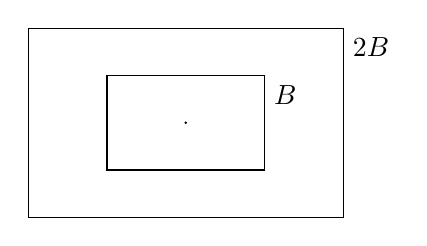
\begin{tikzpicture}[scale=0.4]
    \draw (-2.5,-1.5) rectangle (2.5,1.5) node [below right] {$B$};
    \node [dot, inner sep=0.3pt] {};
    \draw (-5,-3) rectangle (5,3) node [below right] {$2B$};
  \end{tikzpicture}
\end{center}

Hence \hyperlink{def:prog}{$P(x;L)$} is also a $2^r$-approximate group, as is $H + P(x;L)$.
Remarkably, these are essentially the only examples:

\begin{nthm}[Freiman ($G=\mathbb{Z}$); Green-Ruzsa (arbitrary abelian $G$)]\label{thm:5.1}
  Suppose $A \subset G$ (abelian) satisfies $|A+A| \leq K|A|$.
  Then there is a \hyperlink{def:prog}{coset progression} $H+P$ of rank $\leq \mathcal{O}(K^{\mathcal{O}(1)})$ such that
  \begin{equation*}
    A \subset H + P \subset \mathcal{O}(K^{\mathcal{O}(1)}) (A \cup \{0\} \cup -A).
  \end{equation*}
  In particular, \nameref{thm:2.5} gives $|H+P| \leq \exp(\mathcal{O}(K^{\mathcal{O}(1)})) |A|$.
  So $A$ is a large proportion of $H+P$.
\end{nthm}

A substantial part of this result was proved in Introduction to Discrete Analysis, but with a slightly less explicit version of coset progressions.

\begin{defi}
  Let $G$ be a finite abelian group, let
  \begin{equation*}
    \Gamma = \{\gamma_1, \dotsc, \gamma_r\} \subset \hat{G}
  \end{equation*}
  (recall $\hat{G} = \operatorname{Hom}(G,\mathbb{R}/\mathbb{Z})$), and let $p \in [0,\frac{1}{2}]$.
  \hypertarget{def:bohr}Then the set
  \begin{equation*}B(\Gamma,p) = \{g \in G : \forall i\ \norm{\gamma_i(g)}_{\mathbb{R}/\mathbb{Z}} \leq p\}\end{equation*}is called a \named{Bohr set} of rank $r$.
  Here, given $x \in \mathbb{R}/\mathbb{Z}$ with representative $\hat{x} \in (-\frac 12, \frac 12 %)[
  ]$, we write $\|x\|_{\mathbb{R}/\mathbb{Z}} = |\hat{x}|$.
\end{defi}

We will see on Sheet 1 that $\hyperlink{def:bohr}{B(\Gamma,p)}$ is a \hyperlink{def:appGroup}{$4^r$-approximate group}.
Whereas progressions were homomorphic images of boxes, $B(\Gamma,p)$ is the pullback of $[-p,p]^r$ under $(\gamma_1, \dotsc, \gamma_r) \in \hat{G}^r$.

It turns out that the notions of coset progression and Bohr set are essentially equivalent. In Sheet 2, we will see that every coset progression is a Freiman image of a Bohr set of the same rank.
Moreover, every Freiman image of a Bohr set is a large proportion of some coset progression.
We will see a special case of that shortly.

\begin{nprop}\label{prop:5.2}
  Suppose $A \subset G$ (abelian) with $|A+A| \leq K|A|$. Then $\exists B \subset 2A - 2A$, a finite abelian group $Z$ with $|Z| \geq |A|$, a set $\Gamma \subset \hat{Z}$ with $|\Gamma| \leq \mathcal{O}(K^{\mathcal{O}(1)})$, some $p \geq \frac{1}{\mathcal{O}(K^{\mathcal{O}(1)})}$, and a \hyperlink{def:fhom}{centered Freiman $2$-isomorphism} $\varphi: B(\Gamma,p) \to B$.
\end{nprop}

`$2A-2A$ contains a large set isomorphic to a \hyperlink{def:bohr}{Bohr set} of bounded rank'.

In Introduction to Discrete Analysis, we saw this in the special case of $G$ torsion-free.
The general case is harder, but nonetheless conceptually very similar, so we will assume this result from now on.

To pass from \cref{prop:5.2} to \cref{thm:5.1}, we use the following results.

\begin{nprop}\label{prop:5.3}
  Suppose $G$ is a finite abelian group, $\Gamma \subset \hat{G}$ is of size $r$, $p < \frac{1}{10}$.
  Then there is a \hyperlink{def:prog}{coset progression} $H+P \subset B(\Gamma,p)$ with rank $r$ and
  \begin{equation*}
    |H+P| \geq \left(\frac pr\right)^r |G|.
  \end{equation*}
\end{nprop}
\begin{nlemma}\label{lem:5.4}
  Suppose $H+P$ is a \hyperlink{def:prog}{coset progression} of rank $r$, and $\varphi: H + P \to G$ (abelian) is a \hyperlink{def:fhom}{centered Freiman $2$-homomorphism}.
  Then $\varphi(H+P)$ is also a coset progression of rank $r$.
\end{nlemma}
\begin{proof}
  Exercise: If $H$ a group and $\varphi:H \to G$ is a centered Freiman 2-homomorphism, then $\varphi$ is also a group homomorphism.
  In particular, in this lemma $\varphi(H)$ is a finite subgroup. Therefore sufficient to show that
  \begin{equation*}
    \varphi(H + P(x;L)) = \varphi(H) + P(\varphi(x_1), \dotsc, \varphi(x_i); L_1, \dotsc, L_r).
  \end{equation*}
  In fact, we will show that $\forall h \in H$, $|l_i| \leq L_i$ we have
  \begin{equation}
    \varphi(h+l_1 x_1 + \dotsb + l_r x_r) = \varphi(h) + l_1 \varphi(x_1) + \dotsb + l_r \varphi(x_r).\label{eq:5.1}
  \end{equation}
  Since $\varphi$ centered, $\varphi(-x_i) = -\varphi(x_i)$, so we may assume $l_i \geq 0 \ \forall i$.
  Also \eqref{eq:5.1} is trivial if $l_i = 0 \ \forall i$, so may assume $\exists l_j > 0$. Then
  \begin{align*}
    \varphi(h + l_1 x_1 + \dotsb + l_r x_r) &= \varphi(h + l_1 x_1 + \dotsb + l_r x_r) + \varphi(0) \\
                                            &= \varphi(h + l_1 x_r + \dotsb + (l_j-1) x_j + \dotsb + l_r x_r) + \varphi(x_j)
  \end{align*}
  so the result follows by induction on $\sum_i l_i$.
\end{proof}
\begin{proof}[Proof of \cref{thm:5.1}]
  By \cref{prop:5.2} and \cref{prop:5.3} and \cref{lem:5.4}, $\exists H+P$ a coset progression of rank $\leq \mathcal{O}(K^{\mathcal{O}(1)})$ such that $H+P \subset 2A - 2A$ and $|H+P| \geq \exp(-\mathcal{O}(K^{\mathcal{O}(1)}))|A|$.
  We will now apply a version of Ruzsa's covering lemma due to Chang.

  Define recursively sets $S_1, S_2, \dotsc \subset A$ such that $S_i$ is a maximal subset of size $\leq 2K$ such that the translates
  \begin{equation*}
    x + S_{i-1} + \dotsb + S_1 + H + P \quad x \in S_i
  \end{equation*}
  are all disjoint. If ever $|S_i| < 2K$ we stop.
  Now suppose we get as far as $S_1, \dotsc, S_t$. Then
  \begin{equation*}
    S_t + \dotsc + S_1 + H + P \subset 2A - 2A + tA,
  \end{equation*}
  so \cref{thm:2.5} gives
  \begin{equation*}
    |S_t + \dotsb + S_1 + H + P| \leq K^{4+t} |A|.
  \end{equation*}

  On the other hand, disjointness of the translates in the definition of $S_i$ means that
  \begin{align*}
    |S_t + \dotsb + S_1 + H + P| &\geq |S_t| \dotsm |S_1| |H+P| \\
                                 &\geq (2K)^{t-1} \exp(-\mathcal{O}(K^{\mathcal{O}(1)}))|A|.
  \end{align*}
  Putting these together, we have $2^{t-1} \leq K^5 \exp(\mathcal{O}(K^{\mathcal{O}(1)}))$, hence $t \leq \mathcal{O}(K^{\mathcal{O}(1)})$. In particular, this process terminates.
  But also, since $S_t$ is therefore maximal among all subsets of $A$ such that
  \begin{equation*}
    x + S_{t-1} + \dotsb + S_1 + H +P
  \end{equation*}
  are disjoint for $x \in S_t$, Ruzsa's covering lemma implies that
  \begin{equation*}
    A \subset H + 2P + S_1 - S_1 + \dotsb + S_{t-1} - S_{t-1} + S_t.
  \end{equation*}
  Enumerating $\bigcup_i S_i$ as $S_1, \dotsc, S_d$, we have $d \leq \mathcal{O}(K^{\mathcal{O}(1)})$ and
  \begin{equation*}
    A \subset H + 2P + P(s_1, \dotsc, s_d; 1, \dotsc, 1) \subset \mathcal{O}(K^{\mathcal{O}(1)})(A \cup \{0\} \cup -A)
  \end{equation*}
  as claimed.
\end{proof}
\begin{ex}
  See what bounds are given if you apply Ruzsa's covering lemma directly, instead of Chang's argument.
\end{ex}

% new lec
\clearpage
\section{Geometry of Numbers}
\newlec
To prove \cref{prop:5.3}, we'll use a field called the \emph{geometry of numbers} which is concerned with lattices in $\mathbb{R}^d$.
For us, a lattice $\Lambda \subset \mathbb{R}^d$ will simply be the additive subgroup (not subspace) generated by some basis $x_1, \dotsc, x_d$ for $\mathbb{R}^d$.
So
\begin{align*}
  \Lambda = \{l_1 x_1 + \dotsb + \lambda_d x_d \mid l_i \in \mathbb{Z}\}
\end{align*}
If $\Gamma \subset \Lambda$ is another lattice ew call it a sublattice, and write $\Gamma < \Lambda$.
On sheet two, we will see
\begin{equation}
  \frac{\det(y_1, \dotsc, y_d)}{\det(x_1, \dotsc, x_d)} = [\Lambda: \Gamma] \label{eq:6.1}
\end{equation}
where $y_1, \dotsc, y_d$ are a basis for $\Lambda$ and $x_1, \dotsc, x_d$ are a basis for $\Gamma$.

In particular, if $x_1, \dotsc, x_d$ and $x_1', \dotsc, x_d'$ are bases for the same lattice $\Lambda$ then
\begin{equation*}\det(x_1, \dotsc, x_d) = \det(x_1', \dotsc, x_d').\end{equation*}
We define this to be $\det(\Lambda)$.
The relevance of lattices to \cref{prop:5.3} is the following:
\begin{nlemma}\label{lem:6.1}
  Let $G,\Lambda$ be as in \cref{prop:5.3}, and set $\gamma: G \to \mathbb{R}^d/\mathbb{Z}^d$ by enumerating $\Gamma$ as $\{\gamma_1, \dotsc, \gamma_d\}$ and setting $\gamma = (\gamma_1, \dotsc, \gamma_d)$.
  Then $\Lambda = \gamma(G) + \mathbb{Z}^d$ is a lattice with determinant $\ratio{\ker \gamma}{G}$.
\end{nlemma}
\begin{proof}
  $\Lambda$ is finitely generated as $G$ is finite, and torsion-free as in $\mathbb{R}^d$, so isomorphic to $\mathbb{Z}^k$ for some $k$.
  Also, $\Lambda$ has $\mathbb{Z}^d$ as a finite-index subgroup. So $k=d$ and $\spn_\mathbb{R}(\Lambda) = \mathbb{R}^d$.
  So we may take a generating set for $\Lambda$ of size $d$, which is then a basis for $\mathbb{R}^d$. Determinant follows from \eqref{eq:6.1} because $\det(\mathbb{Z}^d) = 1$.
\end{proof}
We'll investigate the interaction of $[-p,p]^d$ with $\Lambda$. To do this, we introduce another definition:
\begin{defi}
  A set $A \subset \mathbb{R}^d$ is convex if $\forall x \in \mathbb{R}^d \setminus A^\circ$ there is a hyperplane $h_x$ with $x \in h_x$ and $h_x \cap A^\circ = \emptyset$.
\end{defi}
\begin{center}
  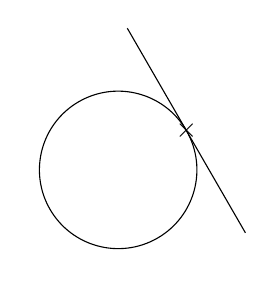
\begin{tikzpicture}[rotate=120]
    \draw (0,0) circle (1cm);
    \draw (-1.5,-1) -- (1.5,-1);
    \node at (0,-1) {$\times$};
  \end{tikzpicture}
\end{center}
\begin{defi}
  A set $B \subset \mathbb{R}^d$ is a convex body if it is bounded and convex and $B^\circ \neq \emptyset$. It is symmetric if $\forall x \in B$ we have $-x \in B$.
  Given a symmetric convex body $B$ and a lattice $\Lambda$, define the successive minima $\lambda_1 \leq \dotsb \leq \lambda_d$ of $B$ with respect to $\Lambda$ via
  \begin{align*}
    \lambda_i = \inf\{\lambda > 0 \mid \dim \spn_\mathbb{R}(\lambda \cdot B \cap \Lambda) \geq i\}
  \end{align*}
\end{defi}
We may then inductively define linearly independent vectors $v_1, \dotsc, v_d \in \Lambda^1$ such that $v_1, \dotsc, v_i \in \lambda_i \bar{B}$.
We'll call such a set a directional basis for $\Lambda$ with respect to $B$. Note $i$ is not unique, and not necessarily a basis for $\Lambda$ in the earlier sense (See Ex Sheet 2).
\begin{nthm}[Minkowski's Second Theorem]\label{thm:6.2}
    Suppose $B$ is a symmetric convex body, $\Lambda$ a lattice in $\mathbb{R}^d$ and $\lambda_1, \dotsc, \lambda_d$ are the successive minima.
    Then $\lambda_1 \dotsm \lambda_d \operatorname{vol}(B) \leq 2^d \det(\lambda)$.
\end{nthm}
\begin{nlemma}[Blichfeldt]\label{lem:6.3}
  Suppose $A \subset \mathbb{R}^d$ is a measurable set, $\Lambda$ a lattice and $\forall a,b \in A$ distinct we have $a-b \notin \Lambda$.
  Then $\operatorname{vol}(A) \leq \det(\Lambda)$.
\end{nlemma}
\begin{proof}
  Fix a basis $x_1, \dotsc, x_d$ for $\Lambda$ and define the \named{fundamental parallelopiped} $P$ with respect to $x_1, \dotsc, x_d$ via
  \begin{align*}
    P = \{l_1 x_1 + \dotsb + l_d x_d \mid l_i \in [0,1)\}
  \end{align*}
  Since $x_1, \dotsc, x_d$ is a basis for $\mathbb{R}^d$, $\forall v \in \mathbb{R}^d$ there are unique $x_v \in \Lambda$ and $p_v \in P$ such that $v = x_v + p_v$.
  Define a map $\varphi:\mathbb{R}^d \to P$ via $\varphi(v) = p_v$.
  This cuts $A$ into countably many measurable pieces, and translates these pieces into $P$.
  It is injective by hypothesis, hence volume preserving, and so
  \begin{equation*}
    \vol(A) = \vol(\varphi(A)) \leq \vol(P) = \det(\Lambda). \qedhere
  \end{equation*}
\end{proof}
\begin{proof}[Proof of \cref{thm:6.2}]
  Let $v_1, \dotsc, v_d$ be a directional basis for $\Lambda$ with respect to $B$. Set $V_i = \spn_\mathbb{R}(v_1, \dotsc, v_i)$ (including $V_0 = \{0\}$), and set $\Lambda_i = \Lambda \cap (V_i \setminus V_{i-1})$.
  $\Lambda$ is a disjoint union $\bigcup_{i=0}^d \Lambda_i$.

  \textbf{Claim 1}: We have $\lambda_d B^\circ \cap (\lambda_d B^\circ + \alpha x) = \emptyset$ whenever $x \in \Lambda_j$ and $\alpha \geq \frac{2\lambda_d}{\lambda_j}$.

  \textbf{Proof of claim} Given $x \in \Lambda_j$, by definition $x \notin \lambda_j B^\circ$, so by convexity there is a hyperplane $h_x$ such that $x \in h_x$ and $H_x \cap \lambda_j B^\circ = \emptyset$.
  By symmetry, we may take $h_{-x} = -h_x$.
  \begin{center}
    \begin{tikzpicture}[xscale=0.7, yscale=1.3]
      \begin{scope}[rotate=-20]
      \draw (0,0) circle (2cm);
      \draw (-2,-2) -- (4,-2);
      \draw (-2,2) -- (4,2);
      \node [dot, label=below:$x$] at (0,2) {};
      \node [dot, label=below:$-x$] at (0,-2) {};
      \node [above] at (3,2) {$h_x$};
      \node [below] at (3,-2) {$-h_x$};
      \end{scope}
    \end{tikzpicture}
  \end{center}
  Note, however, that $-h_x = h_x - 2x$. That means that $x_j B^\circ$ is contained in the slice of space $S_x$ between the parallel hyperplanes $h_x$ and $h_x - 2x$. Clearly $S_x \cap (S_x + \alpha x) = \emptyset$ for all $\alpha \geq 2$, so in particular
  \begin{equation*}
    \lambda_jB^\circ \cap (\lambda_j B^\circ + \alpha x) = \emptyset
  \end{equation*}
  for all such $\alpha$ as well. Scaling by $\lambda_d/\lambda_j$, we see that $\lambda_d B^\circ \cap (\lambda_d B^\circ + \alpha x) = \emptyset$ whenever $\alpha \geq 2 \frac{\lambda_d}{\lambda_j}$, proving the claim. $\blacksquare$

  \textbf{Claim 2}: There are sets $B_1 \subset B_2 \subset \dotsb \subset B_d = \lambda_d B^\circ$ such that
  \begin{enumerate}
    \item $\vol(B_i) = (\frac{\lambda_i}{\lambda_{i+1}})^i \vol(B_{i+1})$ $\forall i$
    \item we have $B_i \cap (B_i + \alpha x) = \emptyset$ whenever $x \in \Lambda_j$ and $\alpha \geq 2 \max\{\frac{\lambda_i}{\lambda_j}, 1\}$. $B_i \cap (B_i + \alpha x) = \emptyset$ whenever $x \in \Lambda_j$ and $\alpha \geq 2 \max\{\frac{\lambda_i}{\lambda_j}, 1\}$. $B_i \cap (B_i + \alpha x) = \emptyset$ whenever $x \in \Lambda_j$ and $\alpha \geq 2 \max\{\frac{\lambda_i}{\lambda_j}, 1\}$. $B_i \cap (B_i + \alpha x) = \emptyset$ whenever $x \in \Lambda_j$ and $\alpha \geq 2 \max\{\frac{\lambda_i}{\lambda_j}, 1\}$.
  \end{enumerate}

  \textbf{Proof of claim 2}: Define operations $\sigma_1, \dotsc, \sigma_{d-1}$ on suitable subsets of $\mathbb{R}^d$ as follows.
  Given $L$ bounded and open, define $\sigma_i$ separately on each affine subspace $z + V_i$ with $z \in L$.
  For each affine subspace, fix a particular $z \in L$, and define
  \begin{align*}
    \varphi(z+v) = z + \frac{\lambda_i}{\lambda_{i+1}} v\quad \forall v \in V_i
  \end{align*}
  On each slice, $\sigma_i$ scales $L$ by a factor of $\frac{\lambda_i}{\lambda_{i+1}}$, centred at $z$ parallel to $v_i$.
  Note the following properties
  \begin{enumerate}[label=(\roman*)]
    \item $\vol(\sigma_i(L)) = (\frac{\lambda_i}{\lambda_{i+1}}) \vol(L)$ (by Fubini)
    \item If $L \cap (z + V_i)$ is open and convex for every $z$, then $\sigma_i(L) \subset L$ because $z \in L$.
    \item If $L \cap (z + V_i)$ is open and convex then so is $\sigma_i(L) \cap (z + V_i)$, and indeed so is $\sigma_i(L) \cap \bigcap_{j < i} (z + V_j)$
  \end{enumerate}
  Set $B_d = \lambda_d B^\circ$, and $B_i = \sigma_i(B_{i+1})$ otherwise.

  Conclusion 1 is immediate from property (i). Conclusion 2 follows from Claim 1 when $i=d$.
  For $i < d$, it follows by induction and repeated application of (ii) and (iii).
  Indeed, (2) for $i \geq j$ follows from (2) for $i+1$ because $\sigma_i$ scales by $\frac{\lambda_i}{\lambda_{i+1}}$ in direction $x$.
  For $i < j$, it follows from $B_i \subset B_{i+1}$. $\blacksquare$

  To prove the theorem, note that $\vol(B_i) = \lambda_i \dotsm \lambda_d \vol(B)$ and by 2, $a - b \notin 2\Lambda$ for every $a,b \in B_1$, so Blichfeldt gives $\vol(B_1) \leq 2^d \det(\Lambda)$.
\end{proof}

% possibly missing stuff
\begin{proof}[Proof of \cref{prop:5.3}]
\newlec
  Write $\gamma = (\gamma_1, \dotsc, \gamma_r) \in \hat{G}^r$, define $\Lambda = \gamma(4) + \mathbb{Z}^r$, which is a lattice of determinant $\ratio{\ker \gamma}{G}$ by \cref{lem:6.1}.
  Let $\lambda_1, \dotsc, \lambda_r$ be the successive minima of $[-1,1]^r$ with respect to $\Lambda$, and $v_1, \dotsc, v_r$ a directional basis. Set $L_i = \floor{\frac{p}{r \lambda_i}}$ for each $i$.
  Then $P(v_1, \dotsc, v_r; L_1, \dotsc, L_r) \subset [-p,p]^r$. Pick for each $i$, pick $x_i \in G$ such that $\gamma(x_i) = v_i$, and set $H = \ker \gamma$.
  Write $p = P(x_1, \dotsc, x_r; L_1, \dotsc, L_r)$. Then $H+P \subset $

  \textbf{Claim}: If $l_1, \dotsc, l_r$ and $l_1', \dotsc, l_r'$ satisfy $|l_i|, |L_i'| \leq L_i$, and
  \begin{equation}
    l_1 x_1 + \dotsb + l_r x_r \in l_1' x_1 + \dotsb + l_r' x_r + H \label{eq:7star} \tag{$*$}
  \end{equation}
  then in fact $l_i = l_i'$ for all $i$.
  Indeed, \eqref{eq:7star} implies that
  \begin{align*}
    (l_1 - l_1') v_1 + \dotsb + (l_r - l_r') v_r \in \mathbb{Z}^r \cap [-2p,2p]^r.
  \end{align*}
  But since $p < \frac{1}{2}$, this last intersection is just $\{0\}$, proving the claim (as $v_i$ are linearly independent in $\mathbb{R}^r$). $\blacksquare$

  Then
  \begin{align*}
    |H+P| &\geq |H|(L_1 +1)\dotsm(L_r+1) \\
          &\geq |H| \left(\frac{p}{r}\right)^r \frac{1}{\lambda_1 \dotsm \lambda_r} \\
          &\geq |G| \left(\frac{p}{r}\right)^r
  \end{align*}
  by Minkowski's second theorem.
\end{proof}

\clearpage
\section{Progressions in the Heisenberg group}
Let
\begin{align*}
  H(\mathbb{Z}) =
  \begin{pmatrix}
    1 & \mathbb{Z} & \mathbb{Z} \\ 0 & 1 & \mathbb{Z} \\ 0 & 0 & 1
  \end{pmatrix} =
  \left\{
    \begin{pmatrix}
      1 & n_1 & n_2 \\ 0 & 1 & n_1 \\ 0 & 0 & 1
    \end{pmatrix}
    : n_i \in \mathbb{Z}
  \right\}
\end{align*}
be the \named{Heisenberg group}.

Set
\begin{equation*}
  u_1 = \begin{pmatrix}
    1 & 0 & 0 \\ &1&1\\&&1
  \end{pmatrix},
  u_2 = \begin{pmatrix}
    1 & 1 & 0 \\ &1&0\\&&1
  \end{pmatrix},
  u_3 = \begin{pmatrix}
    1 & 0 & 1 \\ &1&0\\&&1
  \end{pmatrix}
\end{equation*}
and note that any element of $H(\mathbb{Z})$ can be expressed in the form
\begin{equation*}
  \begin{pmatrix}
    1 & n_2 & n_3 \\ &1&n_1 \\ &&1
  \end{pmatrix}= u_1^{n_1} u_2^{n_2} u_3^{n_3}
\end{equation*}
and we have the following formula for multiplying elements in this form:

\begin{equation}
  (u_1^{n_1} u_2^{n_2} u_3^{n_3})(u_1^{n_1'} u_2^{n_2'} u_3^{n_3'}) = u_1^{n_1+n_1'} u_2^{n_2+n_2'} u_3^{n_3+n_3'+n_1'n_2} \label{eq:7.1}
\end{equation}
This is easy to verify by multiplying matrices, but there is a more abstract reason for it. To see this, given $x,y \in G$, define the commutator $[x,y] = x^{-1} y^{-1} x y$.
In light of the identity $xy = yx [x,y]$, we can view the commutator as being the `error' or `cost' incurred when interchanging two elements.
For example, the fact that commutators are trivial in abelian groups can be viewed as capturing the notion that elements can be interchanged freely in an abelian group.
The $n_1' n_2$ term in \eqref{eq:7.1} arises because we swap the order of $n_1' n_2$ pairs of elements $u_1$ and $u_2$.

Now let's see one possible generalisation of progression to non-abelian groups.
\begin{defi}
  Given $x_1, \dotsc, x_r \in G$, $L_1, \dotsc, L_r \geq 0$, we define the \named{ordered progression} of rank $r$
  \begin{equation*}
    P_{\text{ord}}(x,L) = P_{\text{ord}}(x_1, \dotsc, x_r; L_1, \dotsc, L_r) = \{x_1^{l_1} \dotsm x_r^{l_r} : |l_i| \leq L_i\ \forall i\}.
  \end{equation*}
\end{defi}
Now consider $P=P_{\text{ord}} (u_1, u_2', L_1, L_2)$ for $u_1, u_2 \in H(\mathbb{Z})$ as before, and $L_1, L_2 \geq 0$.
We have
\begin{equation}
  (u_1^{l_1} u_2^{l_2}) (u_1^{l_1'} u_2^{l_2'}) = u_1^{l_1+l_1'} u_2^{l_2+l_2'} u_3^{l_1'l_2} \label{eq:7.2}
\end{equation}
and it is then easy to check that $\ratio{P^2}{P} \to \infty$ as $L_1, L_2 \to \infty$, essentially because by varying $l_1, l_1', l_2, l_2'$ within their ranges one can change $l_1 l_2'$ without changing $l_1 + l_1'$ or $l_2 + l_2'$.
This can be thought of as an extra degree of freedom in $P^2$ compared to $P$.
Coming back to commutators and recalling that $u_3 = [u_2, u_1]$, we see that this corresponds to the freedom to interchange the order of some of the $u_1, u_2$ in $P^2$, as seen in the LHS of \eqref{eq:7.2}.
This is a freedom that the definition of ordered progression explicitly denies us.

It turns out that if we introduce this freedom to $P$ as well then this does force $P$ to have small tripling.

\begin{defi}
  Given $x_1, \dotsc, x_r \in G$, $L_1, \dotsc, L_r \geq 0$, the \named{nonabelian progression} $P(x;L)$ of rank $r$ is defined to consist of those elements of $G$  expressible as products of $x_1^{\pm 1}, \dotsc, x_r^{\pm 1}$ in which each $x_i, x_i^{-1}$ appear at most $L_i$ times between them.
\end{defi}
It turns out $P(u_1, u_2, L_1, L_2)$ does have small tripling (Example Sheet 2).

A note of caution: nonabelian progressions don't always have small tripling; consider $P(x_1, x_2; L_1, L_2)$ for $x_1, x_2$ generators of a nonabelian free group.
In the case of $H(\mathbb{Z})$, the formula \eqref{eq:7.1} is simplified by the fact that $u_3=[u_2, u_1]$ is central in $H(\mathbb{Z})$.
If this were not the case, we'd end up with elements of the form $[[u_2, u_1], u_1]$, for example.
This is in fact a specific example of a property called nilpotence.

To define this, first define a normal series for a group $G$ to be a sequence
\begin{align*}
  G = G_1 > G_2 > \dotsb
\end{align*}
of normal subgroups $G_i \lhd G$, and a central series to be such a normal series in which each $G_i / G_{i+1}$ is central in $G/G_{i+1}$.
\begin{defi}
  A group $G$ is \named{nilpotent} if there is a finite central series
  \begin{align*}
    G = G_1 > \dotsb > G_{s+1} = \{1\}
  \end{align*}
  The smallest $s$ for which such a series exists is called the step or nilpotency class of $G$.
\end{defi}
\begin{ex}
  $H(\mathbb{Z})$ is $2$-step nilpotent.
\end{ex}

\clearpage
\section{Nilpotent Groups}
\newlec
The reasons we focus on nilpotent groups are twofold: there is a clean generalization of Freiman-Green-Ruzsa to nilpotent groups, and a deep theorem of Breuillard, Green and Tao essentially reduces the general case to the nilpotent case.

Given $x_1, \dotsc, x_k \in G$, define the simple commutator
$[x_1, \dotsc, x_k] = [x_1, \dotsc, x_k]_t$ recursively as follows:
\begin{align*}
  [x_1] &= x_1 \\
  [x_1, \dotsc, x_k] &= [[x_1, \dotsc, x_{k-1}], x_k]
\end{align*}
(recall $[x,y] = x^{-1} y^{-1} x y$).

Given subgroups $H,N < G$, define $[H,N] = \langle [h,n] \mid h \in H, n \in N \rangle$, and then given $H_1, \dotsc, H_k < G$, set
\begin{align*}
  [H_1] &= H_1 \\
  [H_1, \dotsc, H_k] &= [[H_1, \dotsc, H_{k-1}], H_k].
\end{align*}
Note that
\begin{equation}
  [H,N] = [N,H] \label{eq:8.1}
\end{equation}
since $[h,n] = [n,h]^{-1}$.

\begin{nlemma}\label{lem:8.1}
  Let $H_1, \dotsc, H_k, N \lhd G$, let $S_i$ be a generating set of $H_i$ for each $i$.
  Suppose $[s_1, \dotsc, s_k] \in N$ whenever $s_i \in H_i$ for each $i$. Then $[H_1, \dotsc, H_k] < N$.
\end{nlemma}
\begin{proof}
  Case $k=1$ is trivial, so assume $k > 1$.
  If $[s_1, \dotsc, s_k] \in N$ for each $s_i \in S_i$ then we have $[[s_1, \dotsc, s_{k-1}], s_k] \in N$ for each $s_i \in S_i$, and hence $[s_1, \dotsc, s_{k-1}] \in C_{G/N}(H_k) = \{g \in G \mid [g,h] \in N \forall h \in H_k\}$.
  The centraliser of a normal subgroup is itself normal, so by induction we have $[H_1, \dotsc, H_{k-1}] \subset C_{G/N}(H_k)$, and hence $[H_1, \dotsc, H_k] \subset N$, as claimed.
\end{proof}
\begin{defi}
  Given a group $G$, we define the \named{lower central series} $G = G_1 > G_2 > \dotsb$ of $G$ via
  \begin{align*}
    G_k \coloneqq \langle [g_1, \dotsc, g_k] \mid g_i \in G\rangle.
  \end{align*}
\end{defi}
Note that $G_k > G_{k+1}$, because $[g_1, \dotsc, g_{k+1}] = [[g_1, g_2], g_3, \dotsc, g_{k+1}]$.
Also, since $[g_1, \dotsc, g_k]^h = [g_1^h, \dotsc, g_k^h]$, each $G_k$ is normal in $G$ (recall $x^y = y^{-1} x y$).
The fact that this is a central series (i.e.\ $G_k/G_{k+1}$ is central in $G/G_{k+1}$) follows from the following result.

\begin{nprop}\label{prop:8.2}
  We have $G_{k+1} = [G_k,G]$ for every $k$. In particular, $G_k = [G, \dotsc, G]_k$.
\end{nprop}
\begin{proof}
  First, $G_{k+1}  < [G_k,G]$ by definition.
  The fact that $[G_k,G] \subset G_{k+1}$ follows from \cref{lem:8.1} since $[g_1, \dotsc, g_{k-1}]$ generate $G_k$ and $G_i, G_k, G_{k+1}$ are normal.
\end{proof}
\begin{nprop}\label{prop:8.3}
  Let $G$ be a group generated by $S$, then
  \begin{equation*}
  G_k = \langle [s_1, \dotsc, s_k] G_{k+1} \mid s_i \in S \ \forall i\rangle.
  \end{equation*}
  `$G_k$ is generated mod $G_{k+1}$ by simple commutators of generators'.
\end{nprop}
\begin{proof}
  Note that $[s_1, \dotsc, s_k]^g \in [s_1, \dotsc, s_k] G_{k+1}$ by definition of $G_{k+1}$, so
  \begin{equation*}
  \langle[s_1, \dotsc, s_k] G_{k+1} \mid s_i \in S\rangle
  \end{equation*}
  is normal in $G$.
  Moreover,
  \begin{equation*}
  [s_1, \dotsc, s_k] \in \langle [t_1, \dotsc, t_k] G_{k+1} \mid t_i \in S\rangle
  \end{equation*}
  whenever $s_i \in S$ for every $i$, so \cref{lem:8.1} implies that
  $[G, \dotsc, G]_k \subset \langle [s_1, \dotsc, s_k] G_{k+1} \mid t_i \in S \rangle$.
  \cref{prop:8.2} gives $[G, \dotsc, G]_k = G_k$, so we have $G_k \subseteq \langle [s_1, \dotsc, s_k] G_{k+1} \mid s_i \in S \rangle$.
  The reverse inclusion is immediate.
\end{proof}
\begin{nprop}\label{prop:8.4}
  We have $[G_i, G_j] \subset G_{i+j}$ for every $i,j$.
\end{nprop}
For this we'll need the following commutator identity, which you can check directly:
\begin{equation}
  [x, y^{-1}, z]^y [y,z^{-1},x]^z [z,x^{-1} y]^x = 1. \label{eq:8.2}
\end{equation}
\begin{proof}[Proof of \cref{prop:8.4}]
  The case $j=1$ follows from \cref{prop:8.2}. So we can assume $j > 1$ and, by induction,
  \begin{equation}
    [G_k, G_{j-1}] \subset G_{k+j-1} \forall k. \label{eq:8.3}
  \end{equation}
  Now note that
  \begin{equation}
    [G_i, G_j] = [G_i, [G_{j-1},G]] = [[G,G_{j-1}],G_i]\label{eq:8.4}
  \end{equation}
  by \cref{prop:8.2} and \eqref{eq:8.1}. We also have
  \begin{equation}
    [[G_{j-1}, G_i], G] = [[G_i, G_{j-1}],G] \subset [G_{i+j-1},G] = G_{k+j}. \label{eq:8.5}
  \end{equation}
  by \eqref{eq:8.1}, \eqref{eq:8.3} and \cref{prop:8.2}, and
  \begin{equation}
    [[G_{i+1}, G], G_{j-1}] = [G_{i+1}, G_{j-1}] \subset G_{i+j}.\label{eq:8.6}
  \end{equation}
  by \cref{prop:8.2} and \eqref{eq:8.3}. Given $x \in G$, $y \in G_{j-1}$ and $z \in G_i$, we therefore have
  \begin{align*}
  [x,y,z] &= (([y^{-1}, z^{-1}, x]^z, [z,x^{-1},y^{-1}]^x)^{-1})^y & &\text{by }\eqref{eq:8.2} \\
          &\subset G_{i+j} &&\text{by } \eqref{eq:8.5}\text{ and }\eqref{eq:8.6}.
  \end{align*}
  The proposition follows from \eqref{eq:8.4} and \cref{lem:8.1}.
\end{proof}
\begin{defi}
  Given a group $G$, the upper central series
  \begin{equation*}
  \{1\} = Z_0(G) < Z_1(G) < Z_2(G) < \dotsb
  \end{equation*}
  is defined recursively by setting $Z_{i+1}(G)$ so that $Z_{i+1}(G)/Z_i(G)$ is the centre of $G/Z_i(G)$.
  Note that each $Z_i(G)$ is normal by induction, since the centre of any group is normal.
\end{defi}
\begin{nthm}\label{prop:8.5}
  Let $G = H_1 > H_2 > \dotsb > H_{i+1} = \{1\}$ be a finite central series for $G$ (so $G$ is nilpotent). Then we have $H_i > G_i$ $\forall i = 1, \dotsc, r+1$ and $H_{r+1-i} \subset Z_i(G)$ for every $0 \leq i \leq r$.
\end{nthm}
This justifies the names upper and lower central series:
\begin{equation*}
  \begin{tikzcd}[sep=tiny]
    Z_r(G) & & Z_{r-1}(G) &&&& Z_1(G) & & Z_0(G)\\
    \vge & & \vge  & & & & \vge && \vge\\
    H_1 & > & H_2 & > & \dots & > & H_r & > & H_{r+1}\\
    \vge & & \vge  & & & & \vge && \vge\\
    G_1 & & G_2 & & & & G_r & & G_{r+1}
  \end{tikzcd}
\end{equation*}

\begin{ncor}\label{cor:8.6}
  If $G$ is $s$-step nilpotent, then both the upper and lower central series have length $s+1$.
\end{ncor}
\begin{proof}
  $H_i > G_1$ by definition, so we may assume $i>1$, and then we have
  \begin{align*}
    H_i &\supset [H_{i-1},G] &&\text{central series} \\
        &\supset [G_{i+1},G] &&\text{by induction} \\
        &=G_i &&\text{by \cref{prop:8.2}}.
  \end{align*}
  We also have $Z_0(G) > H_{r+1}$ by definition, so we may assume $i > 0$ and, by inudction, that $H_{r+2-i} \subset Z_{i-1}(G)$.
  But that
  \begin{equation*}
    G/Z_{i-1}(G) = \frac{G/H_{r+2-i}}{Z_i(G)/H_{r+2-i}}
  \end{equation*}
  because $(H_j)$ is a central series, $H_{r+1-i}/H_{r+2-i}$ is central in $G/H_{r+2-i}$, so its image in $G/Z_{i-1}(G)$ in the above quotient is central.
  But the centre of $G/Z_{i-1}(G)$ is $Z_i(G)/Z_{i-1}(G)$, so $H_{r+1-i} \subset Z_i(G)$, as required.
\end{proof}

These results say
\begin{itemize}
  \item $G$ is nilpotent of step $\leq s \iff G_{s+1} = \{1\} \iff Z_s(G) = G$
  \item If $G = \langle s \rangle$, we can verify this just by checking that $[t_1, \dotsc, t_{s+1}] = 1$ for all $t_i \in S$.
  \item If $G$ is nilpotent of step $\leq s$, then any commutator like $[[[q_1, q_2], q_3], [q_4, q_5]]$ with more than $s$ entries is trivial.
\end{itemize}

\clearpage
\section{Torsion-free Nilpotent Approximate Groups: an overview}
\begin{defi}
  \newlec
  If $\langle x_1, \dotsc, x_r \rangle$ is $s$-step nilpotent then the nonabelian progression $P(x;L)$ is called a \named{nilprogression} of rank $r$ and step $s$.
  In this case, we write $P_{\text{nil}}(x;L)$ instead of $P(x;L)$.
\end{defi}

\begin{nprop*}
  Given $r,s \in \mathbb{N}$, $\exists \lambda = \lambda_{r,s}$ such that if $x_1, \dotsc, x_r$ generate an $s$-step nilpotent group and $L_1, \dotsc, L_r \geq \lambda_{r,s}$ then $P_{\text{nil}}(x;L)$ is an $O_{r,s}(1)$-approximate group (the implied constant can depend on $r,s$ but nothing else).
\end{nprop*}
We won't have time to prove this, but we will do a special case on Sheet 2, where we will also see that it is necessary to have $L_i \geq \lambda_{r,s}$.

As in the abelian setting, it turns out that these are essentially the only examples of finite nilpotent approximate groups, apart from genuine subgroups.

\begin{nthm}\label{thm:9.2}
  Let $G$ be $s$-step nilpotent, $A \subset G$ a finite $K$-approximate group.
  Then $\exists H \lhd \langle A \rangle$ and a nilprogression $P_{\text{nil}}$ of rank $\leq K^{O_s(1)}$ such that $A \subset H P_{\text{nil}} \subset A^{K^{O_s(1)}}$. In particular, $|HP_{\text{nil}}| \leq \exp(K^{O_s(1)})|A|$.
\end{nthm}

\begin{remark}
If $K < 2$, the theorem is trivial. For $K \geq 2$, we have $\mathcal{O}(K^{\mathcal{O}(1)}) \leq K^{\mathcal{O}(1)}$ i.e.\ multiplicative constants can be absorbed into exponents.
  So it is not cheating to write $K^{\mathcal{O}(1)}$ instead of $\mathcal{O}(K^{\mathcal{O}(1)})$.
\end{remark}
We won't have time to prove this in full, but in the next few sections we will prove some special cases that contain most of the main ideas.
We will start with the case where $G$ is torsion-free, where \cref{thm:9.2} is originally due to Breuillard and Green (although we will give a different proof).
We start with the following weakened version:
\begin{nthm}\label{thm:9.3}
  Let $G$ be torsion-free $s$-step nilpotent, $A \subset G$ a finite $K$-approximate group.
  Then $\exists$ an ordered progression $P_{\text{ord}}$ of rank $\leq K^{\mathcal{O}_s(1)}$ such that $A \subset P_{\text{ord}} \subset A^{K^{\mathcal{O}_s(1)}}$.
\end{nthm}

The basic idea is to write $A$ as a product of approximate groups of step $\leq s$, and then apply induction to reduce to the step $1$ case, i.e.\ the abelian case, and apply the Freiman-Green-Rusza theorem.
The result we use to do this is as follows:
\begin{nprop}\label{prop:9.4}
  Let $G$ be torsion-free $s$-step nilpotent, $A \subset G$ a finite $K$-approximate group.
  Then $k \leq K^{\mathcal{O}(1)}$, and $K^{\mathcal{O}(1)}$-approximate subgroups $A_1, \dotsc, A_k \subset A^{\mathcal{O}(1)}$ such that $A \subset A_1 \dotsm A_k \subset A^{K^{\mathcal{O}(1)}}$, and $\langle A_i \rangle$ is of step $< s$ for every $i$.
\end{nprop}

\begin{proof}[Proof of \cref{thm:9.3}]
  An easy induction gives $K^{\mathcal{O}_s(1)}$-approximate groups $B_1, \dotsc, B_m \subset A^{\mathcal{O}_s(1)}$ with $m \leq K^{\mathcal{O}_s(1)}$.
  Freiman-Green-Rusza then gives abelian progressions - in particular ordered progressions - $P_1, \dotsc, P_m$, each of rank $\leq K^{\bigO_s(1)}$, such that $B_i \subset P_i \subset B_i^{K^{\bigO_s(1)}}$, and hence $A \subset P_1 \dotsm P_m \subset A^{K^{\bigO_s(1)}}$.
  $P_1 \dotsm P_m$ is an ordered progression of rank $\leq m K^{\bigO_s(1)} \leq K^{O_s(1)}$, so we are done.
\end{proof}
Recall that in proving Freiman-Green-Rusza, we wanted `$A \subset$ small progression', but we first proved `$A^c \supset$ large progression'.
We then used Chang's covering argument to get what we wanted.
We will use a similar approach here, starting with the following:
\begin{nprop}\label{prop:9.5}
  Take $G$ torsion-free nilpotent, $A \subset G$ finite $K$-approximate group.
  Then $\exists r \leq K^{\bigO(1)}$ and $K^{\bigO(1)}$-approximate groups $A_0, A_1, \dotsc, A_r \subset A^{\bigO(1)}$, each generating a group of step $< s$, such that
  \begin{align*}
    |A_0 A_1 \dotsm A_r| \geq \exp(-K^{\bigO(1)})|A|.
  \end{align*}
\end{nprop}
In the next section, we will see that passing from \cref{prop:9.5} to \cref{prop:9.4} is very similar to the Chang covering part of the proof of Freiman-Green-Ruzsa.

In proving \cref{prop:9.5}, we actually use the preliminary version of Freiman-Green-Ruzsa in which $A^c$ contains a large progression.
As we noted in that proof, combining \cref{prop:5.2}, \cref{prop:5.3} and \cref{lem:5.4} gives the following result:

\begin{nthm}[Green-Ruzsa]\label{thm:9.6}
  Let $G$ be abelian and $A \subset G$ be a finite $K$-approximate group.
  Then $\exists H < G$ and $x_1, \dotsc, x_r$ with $r \leq K^{\bigO(1)}$, and $L_1, \dotsc, L_r \in \mathbb{N}$ such that $HP(x;L) \subset A^4$ and
  \begin{align*}
    |HP(x;L)| \geq \exp(-K^{\bigO(1)})|A|.
  \end{align*}
\end{nthm}
We will apply this to \cref{prop:9.5} via the following result:

\begin{nprop}\label{prop:9.7}
  Let $G$ be $s$-step nilpotent and $A \subset G$ a finite $K$-approximate group.
  Write $\pi: G \to G/[G,G]$ for the quotient homomorphism.
  Noting that $G/[G,G]$ is abelian and that $\pi(A)$ is a $K$-approximate group, let $H < G/[G,G]$ and $x_1, \dotsc, x_r \in G/[G,G]$ be as coming from applying \cref{thm:9.6} to $\pi(A)$.
  Then
  \begin{align*}
    \abs{(A^{24} \cap \pi^{-1}(H)) \prod_{i=1}^r(A^{24} \cap \pi^{-1}(\langle x_i \rangle))} \geq \exp(-K^{\bigO(1)})|A|.
  \end{align*}
\end{nprop}
We will prove \cref{prop:9.7} next time. For now, let's see how it implies \cref{prop:9.5}. \cref{prop:4.6} immediately tells us that $A^{24} \cap \pi^{-1}(H)$ and $A^{24} \cap \pi^{-1}(\langle x_i \rangle)$ are $K^{\bigO(1)}$-approximate groups.

It turns out that they also generate subgroups of step $<s$, at least when $G$ is torsion-free.

\begin{nlemma}\label{lem:9.8}
  Let $G$ be $s$-step nilpotent, and write $\pi: G \to G/[G,G]$ as before.
  Then
  \begin{enumerate}[(i)]
    \item $\forall x \in G/[G,G]$, $\pi^{-1}(\langle x \rangle)$ is of step $<s$.
    \item If $H < G/[G,G]$ is a finite subgroup and $G$ is torsion-free, then $\pi^{-1}(H)$ is of step $<s$.
  \end{enumerate}
\end{nlemma}
\begin{nlemma}\label{lem:9.9}
  Let $G$ be an arbitrary group. Then the simple commutator map
  \begin{align*}
    [\cdot, \dotsc, \cdot]_k : G^k &\longrightarrow G_k \\
    (x_1, \dotsc, x_k) &\longmapsto [x_1, \dotsc, x_k]
  \end{align*}
  is a homomorphism in each variable mod $G_{k+1}$.
  Moreover, $[G,G]$ is contained in the kernel of each of these homomorphisms.
\end{nlemma}

In the next section, we will prove this, use it to prove \cref{lem:9.8} (which is also an exercise in the meantime), and prove the outstanding statements from this section.
\clearpage
\section{Torsion-free Nilpotent Approximate Groups: the details}

% lecture 11
\clearpage
\section{\texorpdfstring{$p$}{p}-groups}
In the last two sections, we looked at approximate subgroups of torsion-free nilpotent groups.
Today we'll move on to consider nilpotent groups with elements of finite order.
We won't need the following result, but it motivates this section.
%nonexaminable
\begin{nprop*}\label{prop:11.1}
  A finite group is nilpotent if and only if it is a direct product of $p$-groups.
\end{nprop*}
Given a prime $p$, a $p$-group is a group in which every element has a power of $p$ as its order.
Motivated by \cref{prop:11.1}, we'll focus on $p$-groups.

In the torsion-free setting, we needed to show that a certain subgroup $\pi^{-1}(H)$ was nilpotent of step $< s$, i.e.\ that $[\pi^{-1}(H), \dotsc, \pi^{-1}(H)]_s = \{1\}$.
We did this by showing that $(\pi^{-1}(+1), \dotsc, \pi^{_1}(+1))_s$ was generated by a union of finite subgroups (i.e. the subgroups $[\pi^{-1} H, q_1, \dotsc, q_{s-1}]$ with $g_i \in \pi^{-1}(H)$.)
Since the ambient group was torsion-free, these finite subgroups were all automatically trivial, hence so was $[\pi^{-1}(H), \dotsc, \pi^{-1}(H)]_s$.

This does not work if the ambient group has two elements of finite order, so we need to find a more sophisticated way of controlling groups like $[\pi^{-1}(+1), \dotsc, \pi^{-1}(H)]_s$ that are generated by unions of subgroups.

In this section we will prove the following result giving a means by which to do this.
\begin{nprop}\label{prop:11.2}
  Let $\Gamma$ be a (finite) abelian $p$-group of rank $\leq r$, and let $X \subset \Gamma$ be a union of subgroups. Then $\langle x \rangle \subset r X$.
\end{nprop}

The \named{rank} of a group here is the smallest possible size of a generating set.

Given a group $G$, a subgroup $H < G$ is a \named{maximal subgroup} if $H \neq G$ but the only subgroup $N < G$ satisfying $H \lneqq N < G$ is $G$ itself.
\begin{nlemma}\label{lem:11.3}
  Let $\Gamma$ be a finite abelian $p$-group.
  Then $H < \Gamma$ is maximal iff $\Gamma/H \cong \mathbb{Z}/p\mathbb{Z}$.
\end{nlemma}
\begin{proof}
  The fundamental theorem of finitely generated abelian groups tells us that
  \begin{align*}
    \Gamma/H \cong \bigoplus_{i=1}^k \frac{\mathbb{Z}}{p^{n_i}\mathbb{Z}}
  \end{align*}
  for some $k \geq 0$ and $n_i \in \mathbb{N}$. The lemma follows immediately.
\end{proof}
\begin{nlemma}\label{lem:11.4}
  Let $\Gamma$ be a finite abelian $p$-group, and let $S \subset \Gamma$. Then $S$ generated $\Gamma$ iff $S + (p \cdot \Gamma)$ generates $\Gamma$. (We write $p \cdot \Gamma$ to mean $\{p x : x \in \Gamma\}$).
\end{nlemma}
As a slogan, ``$S$ generates $\Gamma$ $\iff S$ generated $\Gamma/(p \cdot G)$''.

\begin{proof}
  Clearly if $S$ generates $\Gamma$ then so does $S + (p \cdot \Gamma)$.
  Conversely, if $S$ does not generate $\Gamma$ then $S$ is contained in some maximal subgroup $H$.
  We know from \cref{lem:11.3} that $\Gamma/H \cong \mathbb{Z}/p\mathbb{Z}$, so $(p \cdot \Gamma) \subset H$ because $px$ is trivial in $\Gamma/H$ for every $x \in \Gamma/H$.
  Hence $S + (p \cdot \Gamma) \subset H$, so does not generate $\Gamma$.
\end{proof}
\begin{ncor}\label{cor:11.5}
  Let $\Gamma$ be a finite abelian $p$-group. Then every minimal generating set for $\Gamma$ has the same size.
\end{ncor}
\begin{proof}
  The fundamental theorem of finitely generates abelian groups implies that $\Gamma/(p \cdot \Gamma) \cong \mathbb{F}_p^n$.
  \cref{lem:11.4} says that $S$ generates $\Gamma$ iff its image in $\Gamma/(p \cdot \Gamma)$ generates $\mathbb{F}_p^n$.
  A minimal generating set therefore has as its image in $\Gamma/(p \cdot \Gamma)$ a basis for $\mathbb{F}_p^n$, and, moreover, no two elements of $S$ project to the same element of $\Gamma/(p \cdot \Gamma)$.
  Hence $|S|=n$ (which does not depend on $S$).
\end{proof}
\begin{nlemma}\label{lem:11.6}
  Let $\Gamma$ be a finite abelian $p$-group of rank $r$, and suppose $\Gamma' < \Gamma$. Then the rank of $\Gamma'$ is also $\leq r$.
\end{nlemma}
\begin{proof}
  The case $r=0$ is trivial, so we may assume $r > 1$ and proceed by induction.
  We have a generating set $x_1, \dotsc, x_r$ for $\Gamma$. Let $m$ be maximal such that $\Gamma' \subset p^m \cdot \Gamma$.
  Since $p^m \cdot \Gamma$ is generated by $p^m x_1, \dotsc, p^m x_r$, $p^m \cdot \Gamma$ also has rank $\leq r$, so without loss of generality we may replace $\Gamma$ with $p^m \cdot \Gamma$, and hence assume that $\Gamma'$ is not contained in $p \cdot \Gamma$ (by maximality of $m$).

  That means $\exists y \in \Gamma \setminus p \cdot \Gamma$, i.e.\ $y$ is of the form $l_1 x_1 + \dotsb + l_r x_r$ with at least one $l_i$ (WLOG $l_r$) not a multiple of $p$.
  That means that $l_r$ has a multiplicative inverse, say $q$, mod the order of $x_r$, and hence
  \begin{align*}
    x_r = q (y - l_1 x_1 - \dotsb - l_{r-1} x_{r-1}).
  \end{align*}
  This means that $\Gamma / \langle y \rangle$ has rank $\leq r-1$ and hence, by induction, so does $\Gamma' / \langle  y \rangle$.
  In particular, $\Gamma'$ has rank $\leq r$ (add $y$ to a generating set for $\Gamma' / \langle y \rangle$).
\end{proof}
\begin{proof}[Proof of \cref{prop:11.2}]
  \cref{lem:11.6} implies that $\langle x\rangle$ has rank $\leq r$, and so \cref{cor:11.5} implies that $\exists x_1, \dotsc, x_r \in X$ such that
  \begin{align*}
    \langle x \rangle = \langle x_1, \dotsc, x_r \rangle = \langle x_1 \rangle + \dotsb + \langle x_r \rangle.
  \end{align*}
  Since $X$ is a union of subgroups, each $\langle x_i \rangle \subset X$, so in fact $\langle x \rangle \subset rX$, as required.
\end{proof}
(Note that $p \cdot \Gamma$ referred to multiplying each element of $\Gamma$ by $p$, and $rX$ refers to higher sumsets as in earlier parts of the course).
\color{gray}
\subsection*{*Bonus content}
We showed in lectures 9 and 10 that if $A$ is a finite $K$-approximate subgroup of a torsion-free nilpotent group then $\exists$ ordered progression $P_{\text{ord}}$ of rank $\leq K^{\mathcal{O}(1)}$ such that $A \subset P_{\text{ord}} \subset A^{K^{\mathcal{O}_s(1)}}$.
However, in the general theorem we had a nilprogression instead.
To get around this, one uses the following result.
\begin{nprop*}\label{prop:11.7}
  Let $x_1, \dotsc, x_r \in G$ (where $G$ is $s$-step nilpotent), and $L_1, \dotsc, L_r \geq 0$.
  Then
  \begin{equation*}
    P_{\text{ord}}(x;L) \subset P_{\text{nil}}(x;L) \subset P_{\text{ord}}(x;L)^{\mathcal{O}_s(r^{\mathcal{O}(s)})}.
  \end{equation*}
\end{nprop*}
\color{black}
\printindex
\end{document}
